\chapter{State of the art}\label{SotA}

Before we get into the problem of motion planning for robotic manipulators, let us take a step back and look at motion planning as a whole. This is arguably the most researched problem in robotics; there have been thousands of research papers with the motion planning keyword published in the recent years~\cite{RASreview}. The motion planning problem goes beyond a specific type of robot, or a specific problem; the term encapsulates movement of a robotic arm, legged robots, autonomous cars and even devices for exploration of oceans and space. It often consists of multiple stages: first a path is found, then velocities necessary to realise the movement are computed, then the movement is realized with potential error handling.

As researchers try to develop new algorithms and push the boundaries of what is computable, there are a few concepts at the core of each method, which are worth taking a look at.

\section{General concepts -- path planning for a 2D robot}

\begin{figure}[ht]
    \centering
    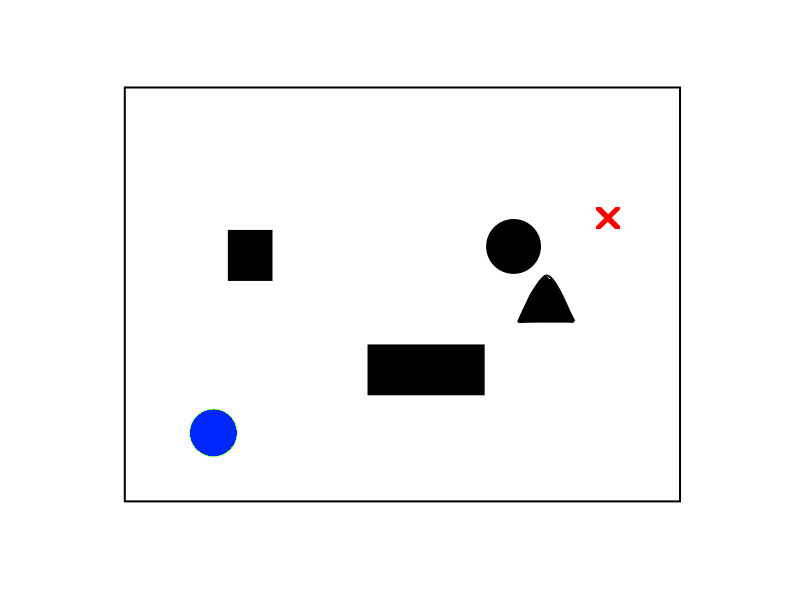
\includegraphics[width=0.4\textwidth]{robot_obstacles.png}
  \caption{A moving robot (blue) in 2 dimensions, trying to reach a target (red) while avoiding obstacles (black).}\label{fig:bot}
\end{figure}

For simplicity, let us consider the case of a robot that can move in any direction, trying to find a path to a goal in a 2-dimensional space with some obstacles. The proper term for this is path planning; since we are only concerned with finding a path and not realising the actual movement, it is a subproblem of motion planning. Though in some literature, the terms are incorrectly used interchangeably.

We will assume that the robot has full knowledge of the environment, and the environment remains unchanging. This is a heavy simplification, as real robots generally have limited ways of movement, and real life environments can often change dynamically. However, this simplified representation lets us easily visualize and understand each of the concepts before discussing their extensions. Each of the concepts can be generalised to higher dimensions and applied to robotic manipulators specifically.

The first idea that comes to mind after completing a basic algorithms course is to use algorithms for finding the shortest paths, such as the asymptotically optimal Djisktra's algorithm. The problem is that the space we are moving in is continuous, while the shortest path graph algorithms require discrete graphs connected with edges.

\begin{figure}[ht]
    \centering
    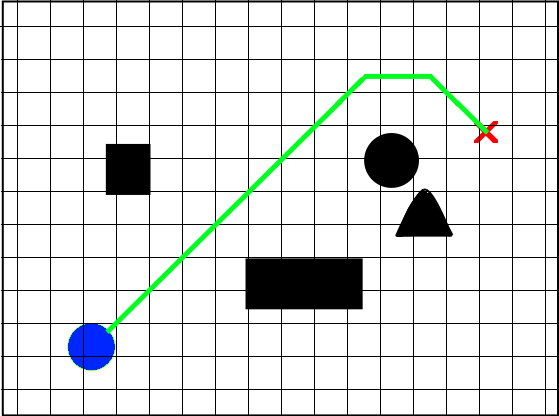
\includegraphics[width=0.4\textwidth]{robot_grid_path.png}
  \caption{Path to target found by Djikstra's algorithm on a grid.}\label{fig:grid}
\end{figure}

An intuitive approach to discretizing our space is creating a grid that represents the space, treating the points on the grid as vertices, and assigning the edges that lead to an occupied square an infinite cost. On this grid, finding the shortest path is a simple task. The main advantages to such an approach are implementational simplicity and easy generalization to 3 dimensions. Further constraints can be implemented using the weights on the grid; for example, when planning the path for a car, the weight on edges can reflect the speed limit on the corresponding road.
This method has been used successfully as a base for motion planning of autonomous vehicles~\cite{grid1, grid2}.

The main problem is choosing the size and shape of the grid. If the spacing between the vertices is too large, the resulting path diverges further from the optimal one, and the algorithm might not find a valid solution in a space with many small obstacles. However, if the spacing is too small, the number of vertices that need to be explored can easily become too large to compute in a reasonable amount of time.


\begin{figure}
  \centering
  \begin{minipage}{0.8\textwidth}
  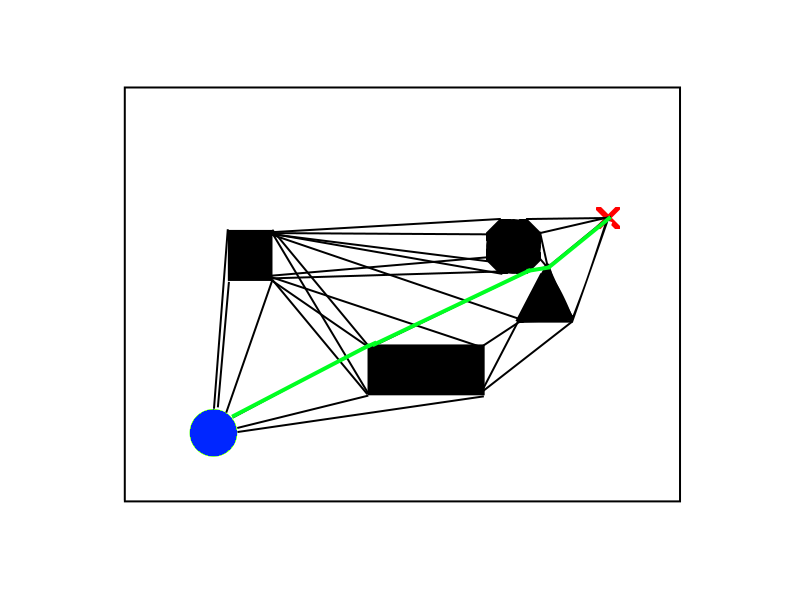
\includegraphics[width=0.5\textwidth]{robot_visibility.png}
  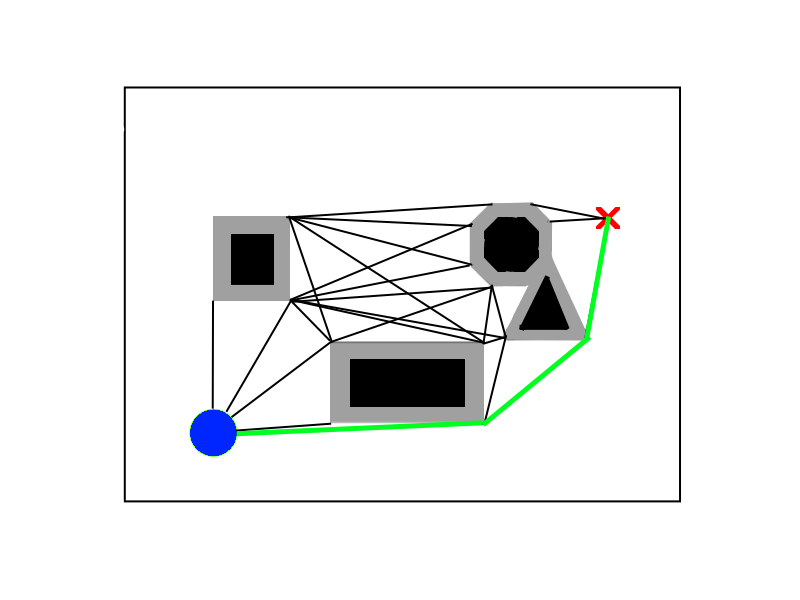
\includegraphics[width=0.5\textwidth]{robot_visibility_ext.png}
  %\caption{Shortest path on a widened visibility graph.}%\label{fig:vis_ext}
  \end{minipage}
  \caption{Shortest path on a visibility graph, before and after widening obstacles.}\label{fig:vis}
\end{figure}

In an effort to reduce the size of our graph and thereby speed up the graph-based path planning methods, visibility graphs have been suggested. To construct a visibility graph, obstacles in the workspace need to be approximated with polygons of choice. The corners of these polygons become the vertices of our graph. Two vertices are connected with an edge if they see each other in the intuitive sense: there is no obstacle on the direct line between them. Each edge is assigned weight corresponding to the euclidean distance of the vertices. Then, standard shortest path algorithms are computed on the graph.

% \begin{figure}
%     \centering
% \end{figure}

As we can see in Figure~\ref{fig:vis}, the basic method can find impossible paths, since it does not account for the size of the robot. The way to mitigate this problem is to extend the size of each obstacle with respect the size and movement limitations of our robot; in the simplified problem, simply expanding each obstacle by the robot's radius is enough. The advantage to this approach is that we can reduce the size of the graph and still find paths close to optimal in the 2D path planning problem. A dynamic extension has also been suggested~\cite{DVG}, which makes the algorithm more flexible in changing environments.

Unfortunately, the method does not scale well to 3 dimensions, as the optimal path rarely leads directly around obstacles. We also need to be wary of imprecisions in the robot's movement; a path close to the obstacles could easily lead to a collision upon a mechanical error. These disadvantages have made the method less popular in recent years.

The opposite approach has been more successful. Rather than considering points as close to the obstacles as possible, we can consider the furthest points from nearby obstacles, and construct a so-called Voronoi diagram. This method provides safe and smooth paths for the robot~\cite{voronoi} and is still used today as a base for modern motion planning algorithms~\cite{voronoi2}. However, much like the previous method, voronoi diagrams are hard to scale to more than 2 dimensions. Therefore, they will not be as useful for our use case.

Regardless of the resulting shape of the graph, the choice of the shortest path algorithm can play a significant role in the path planning problem. Rather than using the traditional Djikstra's algorithm, the modern approach is to use the A* algorithm.

The A* algorithm~\cite{ai_modern} can be viewed as an extension of Djikstra's shortest path algorithms and uses a heuristic which influences what nodes will be chosen during the graph search. Under two conditions, the algorithm is complete\footnote{If a solution exists, the algorithm will find the best one.} and asymptotically optimal. The first condition on the heuristic is admissibility -- the heuristic never overestimates the cost to reach the goal. The second is consistency -- the value estimated by the heuristic is always less than or equal to the estimated distance from any neighbouring vertex to the goal, plus the cost of reaching that neighbour.

Since we are discussing the problem of finding a path to a target, a simple heuristic that is both admissible and consistent is the euclidean distance of a vertex to the target. Exploring vertices based on the distance from the target can often lead to obtaining a much faster solution, but gives us no guarantees on actually being faster than Djikstra.

The disadvantage to using this algorithm is that a suitable heuristic can be hard to find, and the worst case space complexity is higher than for Djikstra's algorithm. Still, the algorithm is widely used and and can be generalized to further problems.

%\newpage
With a precise enough representation of space, graph-based solutions can give us certain guarantees on the optimality of the path. However, discretizing a continuous space can take a lot of memory and computational time.
If we relax the requirement of exploring the whole space and look for faster algorithms that provide \enquote{good enough} solutions, we can move away from graph-based approaches. Gradient based approaches make local decisions based on some criteria, and iteratively move towards the target. Among these, a path planning algorithm that stands out is the Artificial Potential Field (APF) method.


Intuitively, objects in the APF algorithm act on our robot as magnets. The target attracts our robot with a strong force, while the obstacles repulse the robot. In an ideal scenario, this results in finding a smooth path to the target while avoiding obstacles, see~\ref{fig:apf}. This algorithm is highly efficient, and can be extended to various problems. Besides its low cost, one of the main advantages is that the algorithm can quickly react to a changing environment, which makes it more flexible in dynamic environments compared to the graph-based methods.

\begin{figure}[ht]
  \centering
  \begin{minipage}{0.8\textwidth}
    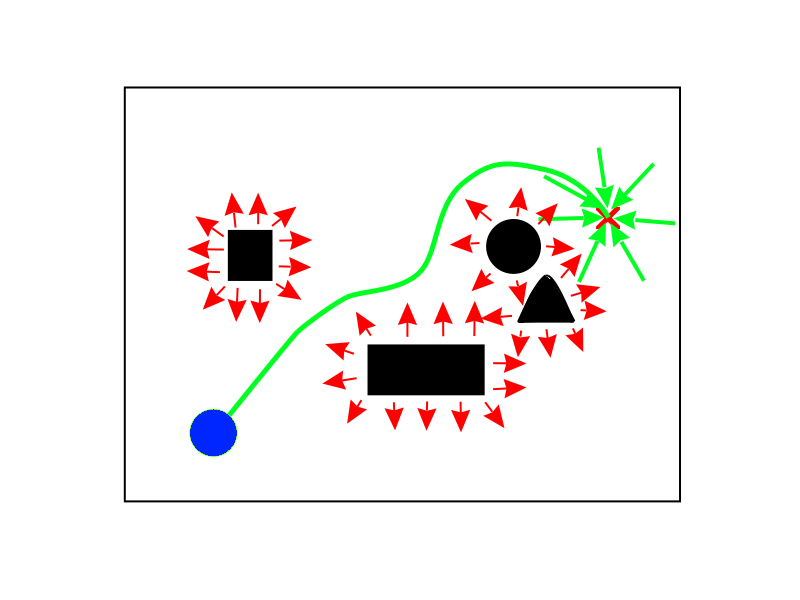
\includegraphics[width=0.5\textwidth]{robot_apf.png}
    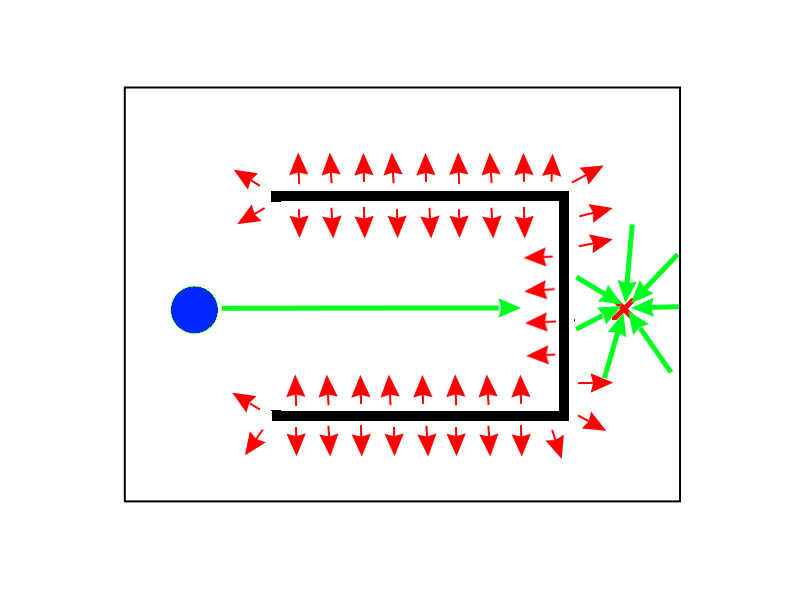
\includegraphics[width=0.5\textwidth]{robot_apf_min.png}
  \end{minipage}
  \caption{APF finds smooth paths, but is susceptible to local minima.}\label{fig:apf}
\end{figure}

There are two main downsides to the algorithm. For one, it gives us no guarantees on the optimality of the found path; but even worse than that, the basic version is susceptible to local minima. Some authors suggest extensions that help the robot get around obstacles~\cite{apf, apf2}, while another common use for the algorithm is to plan a global path using a graph-based method and use APF to make local decisions and move between the found points~\cite{hybrid}. Since this method can easily be generalised to more dimensions, it is quite relevant in today's research.


%\newpage
The last family of algorithms is based on random sampling. Arguably the most popular method used all throughout motion planning is the Rapidly-exploring Random Tree (RRT) algorithm~\cite{LaValle1998RapidlyexploringRT}. In each iteration of the algorithm, a random point in the space is sampled. Then, an edge is created from the nearest node to the sampled point if a valid path exists between them. Each iteration is very fast, hence the space can easily be sampled millions of times. Once a point that allows reaching the target has been found, the algorithm finishes.

\begin{figure}[ht]
  \centering
  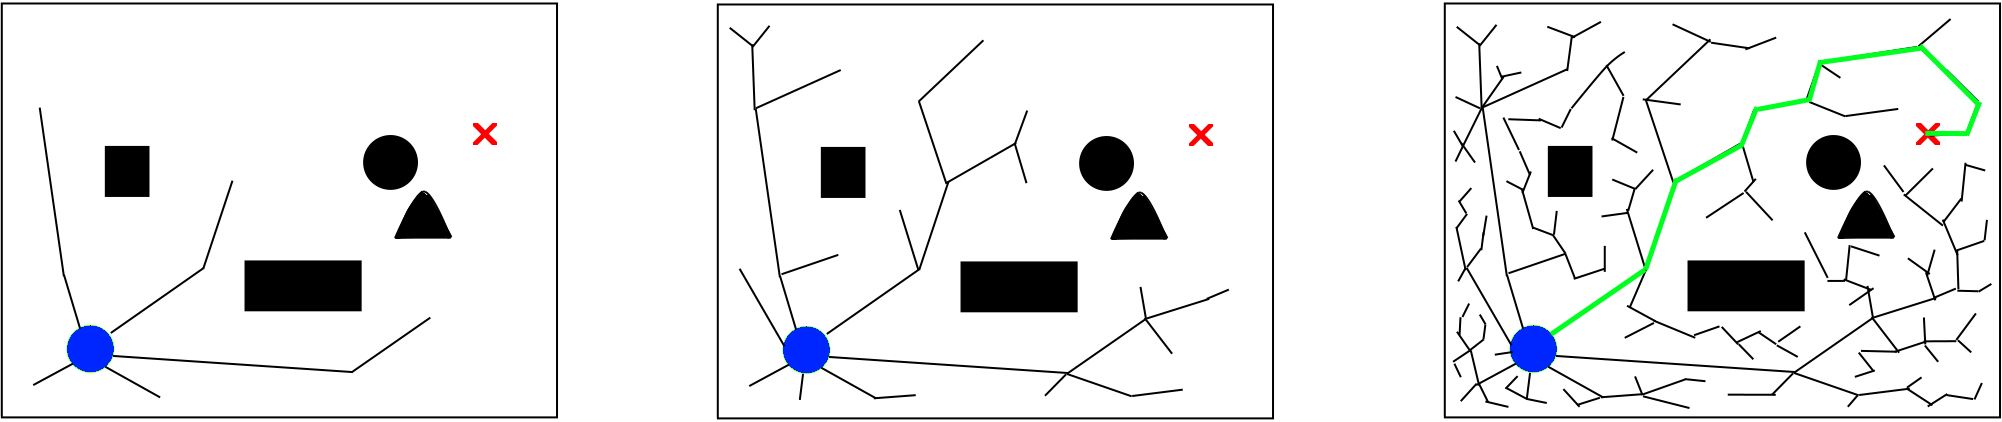
\includegraphics[width=\textwidth]{robot_rrt.png}
  \caption{RRT expanding to reach the target.}
\end{figure}

The RRT algorithm grants no guarantees on how quickly a path will be found, nor does it find optimal paths, but in practice, it performs very well. Countless extensions have been suggested, most notably the RRT* method~\cite{rrt_star}, which continually improves the found paths. Unlike the basic RRT method, if RRT* could run indefinitely, it would find an optimal solution. As a result, we can let the algorithm run for a set amount of iterations and, depending on the task at hand, find the right balance between how quickly we obtain a solution and how good it is.

The main advantage of the RRT methods is their versatility. There are countless variations that place limitations on how to sample the points, how to create new edges, and when to stop. The algorithms can be extended to more dimensions; not only can it trivially be applied in 3 dimensions, we can also define our state space in different ways. If we consider the rotations of a manipulator as our dimensions, the algorithm works just as well for finding a trajectory for a robot manipulator. The downside to this approach is that the state space grows exponentially with each dimension; as a result, it cannot be trivially applied to high-DoF manipulators.

\section{Motion planning of manipulators}

While the 2-dimensional path planning for mobile robots is an interesting problem in itself, we are interested in how the aforementioned methods can be generalised to robotic manipulators.

Remember the initial problem we are trying to solve: given a target in cartesian coordinates, we wish to compute movement of a robotic manipulator so that the end-effector reaches the target position, and the robot avoids any collisions with the environment during the movement.

The key to extending graph-based methods to robotic manipulators is the redefinition of space from cartesian coordinates to the robot's joint parameters. The key to obtaining a target configuration for the manipulator lies in inverse kinematics. First, we can use IK to compute joint parameters of the manipulator so that the end-effector has been reached. As a result, we have a target configuration, and the problem can be defined with respect to the joint parameters.
Since the manipulator's parameters uniquely define the robot's state, the problem of reaching a specific configuration is well defined. Once we've discretized the space of possible joint positions, we can use i.e.\ the A* algorithm to compute a path to the target position. Using forward kinematics, it's easy to determine which positions collide with an obstacle.

By combining the pieces, we can solve the entire problem. A successful application of this method for a 6-DoF industrial robot manipulator can be found here~\cite{doubleA_star}. The authors first compute a 3D model of the surrounding environment, so that collisions can be avoided. They leverage inverse kinematics to compute a position where the target is reached. Then, a path to reaching the target configuration is computed in 2 stages:

\begin{itemize}
\item First, the space is discretized very roughly into 20 segments, to minimize the otherwise enormous state space. A* is used to find a path to a configuration close to the target.
\item Second, a finer discretization is used in a smaller subspace, and the target configuration is reached, once again with A*.
\end{itemize}

Finally, they use a control loop that moves the joints to follow the computed path and correct any mechanical errors.

The method leaves some unanswered questions, but works reasonably well for industrial 6-DoF manipulators. However, we need to keep in mind that an increasing number of joints makes the size of the state space grow exponentially. As a result, if we tried to apply the algorithm beyond 6 dimensions, we would either have to sacrifice a lot of precision by discretizing the space into even larger segments, or not obtain a solution in reasonable time. In a similar fashion, the A* part can be replaced with an RRT-based algorithm, but struggles due to the exponentially rising state space.

On our search for a more scalable algorithm, we can once again look into Artificial Potential Field methods. In this case, the virtual forces don't influence the entire robot; instead, each joint is repulsed by the surrounding obstacles, while the end-effector is pulled in by the target. A solution using this method has been proposed here~\cite{aapf}. The paper deals with the specifics on how to incorporate end effector rotation into the algorithm and avoid local minima. However, the evaluation is far from satisfying. The authors present their solution on a single use case: grabbing an object that lies near another obstacle. The results are fine, but it remains unclear how well the algorithm would work in an environment with many obstacles near the initial joints of the manipulator.

Since the traditional A* and RRT methods with respect to joints do not translate well to higher dimensions, a modern approach is to use RRT to generate a path for the end effector only, and try to reproduce it using the other joints~\cite{RRT_manipulator, rrt_industrial}. However, most of the authors do not consider obstacles close to the base of the manipulator, which makes the results questionable.

A very powerful method is presented in~\cite{rrt_fabrik}. The authors use a RRT algorithm to sample points for the \textit{end effector} in a space filled with obstacles. Then, FABRIK is used to compute whether the new sampled point is reachable from the nearest node without causing a collision, and if it is, it is considered a valid node. This combination of planning with respect to the end effector along with the highly efficient inverse kinematics algorithm is similar to the approach that will be presented in this thesis. Unfortunately, the authors present the algorithm as a manipulator in space, and as a result, make a lot of simplifications in their approach that would not translate as well to real robots.

\begin{itemize}
  \item No effort is made to smooth or optimize the found path, therefore, rather than moving the joints at a constant velocity towards the target, the actual movement would be erratic and highly inefficient.

  \item There is no consideration for joint limits of the manipulator. FABRIK becomes more expensive when joint limits are involved; and while still fast, computing it a million times within RRT would take a very long time. Additionally, when choosing a target for FABRIK in a constrained system, we need to take the end effector rotation into account. How to do this within the RRT remains unanswered.
\end{itemize}

Historically, the idea of planning with respect to the \textit{end effector} and repeatedly computing inverse kinematics for the remainder of the manipulator has been frowned upon, due to the high cost associated with computing the pseudoinverse and other optimization methods. However, this is no longer as big of a concern: with the efficiency of FABRIK, we can afford to compute it many times to make incremental changes along a specific path.
